% Earth's Coordinates -- Guided Notes
% Earth Science
%
% Compile the student copy:
%     pdflatex Earths_Coordinates_Notes.tex
% Compile the answer key:
%     pdflatex -jobname=Earths_Coordinates_KEY "\def\answerkey{}% Earth's Coordinates -- Guided Notes
% Earth Science
%
% Compile the student copy:
%     pdflatex Earths_Coordinates_Notes.tex
% Compile the answer key:
%     pdflatex -jobname=Earths_Coordinates_KEY "\def\answerkey{}% Earth's Coordinates -- Guided Notes
% Earth Science
%
% Compile the student copy:
%     pdflatex Earths_Coordinates_Notes.tex
% Compile the answer key:
%     pdflatex -jobname=Earths_Coordinates_KEY "\def\answerkey{}% Earth's Coordinates -- Guided Notes
% Earth Science
%
% Compile the student copy:
%     pdflatex Earths_Coordinates_Notes.tex
% Compile the answer key:
%     pdflatex -jobname=Earths_Coordinates_KEY "\def\answerkey{}\input{Earths_Coordinates_Notes.tex}"

\documentclass[11pt,addpoints]{exam}

\usepackage[margin=0.85in,top=1.1in,headsep=0.25in]{geometry}
\usepackage{graphicx}
\usepackage{amsmath}
\usepackage{textcomp}
\usepackage{enumitem}
\usepackage{xcolor}
\usepackage{tcolorbox}
\usepackage{parskip}
\usepackage{needspace}

\ifdefined\answerkey
  \printanswers
\fi

% ---------------------------------------------------------------- formatting
\pagestyle{headandfoot}
\firstpageheader{\textbf{Earth's Coordinates}}{}{Name: \makebox[1.6in]{\hrulefill}}
\runningheader{\textbf{Earth's Coordinates}}{}{Name: \makebox[1.6in]{\hrulefill}}
\firstpagefooter{Earth Science}{Page \thepage\ of \numpages}{Date: \makebox[1.1in]{\hrulefill}\ \ Per: \makebox[0.4in]{\hrulefill}}
\runningfooter{Earth Science}{Page \thepage\ of \numpages}{}
\headrule
\footrule

\renewcommand{\thequestion}{\arabic{question}}
\pointsinrightmargin
\bracketedpoints

\newcommand{\dg}{\ensuremath{^{\circ}}}
\newcommand{\mn}{\ensuremath{'}}

% a fill-in blank of standard width
\newcommand{\blank}[1]{\fillin[#1][1.35in]}
\newcommand{\shortblank}[1]{\fillin[#1][0.85in]}
\newcommand{\longblank}[1]{\fillin[#1][2.6in]}
\newcommand{\tblblank}[1]{\fillin[#1][1.2in]}
\newcommand{\midblank}[1]{\fillin[#1][1.1in]}

% open-response prompt: ruled lines for students, answer text for the key
\newcounter{rl}
\newcommand{\responselines}[1]{%
  \setcounter{rl}{0}%
  \loop\ifnum\value{rl}<#1\relax
    \noindent\rule{\linewidth}{0.4pt}\par\vspace{1.15\baselineskip}%
    \stepcounter{rl}%
  \repeat}
\newcommand{\openresponse}[2][2]{%
  \ifdefined\answerkey
    \par\vspace{0.2\baselineskip}\noindent\textbf{#2}\par\vspace{0.4\baselineskip}%
  \else
    \par\vspace{0.6\baselineskip}\responselines{#1}%
  \fi}

\newtcolorbox{keyidea}{
  colback=black!4, colframe=black!55, boxrule=0.6pt,
  left=6pt, right=6pt, top=5pt, bottom=5pt, arc=2pt
}

\newcommand{\sectiontitle}[1]{%
  \needspace{6\baselineskip}%
  \vspace{0.6\baselineskip}%
  \noindent\textbf{\large #1}\par\nopagebreak
  \vspace{-0.4\baselineskip}\noindent\rule{\linewidth}{0.8pt}\par\nopagebreak
  \vspace{0.2\baselineskip}}

% ---------------------------------------------------------------- document
\begin{document}

\begin{center}
  {\Large\textbf{Earth's Coordinates}}\\[2pt]
  {\large Guided Notes \ifdefined\answerkey\textbf{--- ANSWER KEY}\fi}\\[4pt]
  \textit{Driving question: How do we locate things on Earth?}
\end{center}

\vspace{0.4\baselineskip}

% ================================================================
\sectiontitle{1. Why we need a coordinate system}

Directions given by landmark (``two miles past the old barn'') only work if you
already know the landmark. A \textbf{coordinate system} gives every point on Earth
one unique address built from a grid of \blank{intersecting} lines.

\begin{keyidea}
The grid is anchored to something that never moves: Earth's \blank{axis of rotation}.
The poles and the equator come from the way Earth spins, not from a human decision.
\end{keyidea}

% ================================================================
\sectiontitle{2. Latitude and longitude}

Complete the table.

\vspace{0.3\baselineskip}
\renewcommand{\arraystretch}{1.9}
\noindent\begin{tabular}{@{}p{1.5in}p{2.4in}p{2.4in}@{}}
\hline
 & \textbf{Latitude} & \textbf{Longitude} \\
\hline
Lines run\dots & \tblblank{east--west} & \tblblank{north--south} \\
Measured\dots & \tblblank{north--south} & \tblblank{east--west} \\
Do they touch? & \tblblank{no, parallel} & \tblblank{yes, at the poles} \\
Measured from\dots & \tblblank{the equator} & \tblblank{prime meridian} \\
That line is\dots & 0\dg\ latitude & 0\dg\ longitude \\
Range & 0\dg\ to \shortblank{90\dg} N or S & 0\dg\ to \shortblank{180\dg} E or W \\
\hline
\end{tabular}
\renewcommand{\arraystretch}{1}

\vspace{0.5\baselineskip}

\begin{keyidea}
Every coordinate needs \textbf{a number AND a direction}. 43\dg\ is not a location.
43\dg\ N is a line; 43\dg\ N, 76\dg\ W is a point.\\[3pt]
\textbf{Latitude is always written first.}
\end{keyidea}

\vspace{0.3\baselineskip}
\noindent Why does latitude stop at 90\dg\ but longitude go to 180\dg?

\openresponse[2]{At 90\dg\ you have reached the pole --- there is no more Earth to travel.
Longitude can run 180\dg\ each way because you can circle halfway around in either direction.}

% ================================================================
\sectiontitle{3. Degrees and minutes}

When we zoom in, latitude and longitude are given in degrees \textit{and}
\textbf{minutes}, written with a prime symbol (\mn).

\[ 1\dg = \shortblank{60}\mn \qquad 30\mn = \tfrac{1}{2}\dg \qquad 10\mn = \tfrac{1}{6}\dg \]

\begin{itemize}[nosep,leftmargin=1.6em]
  \item Halfway between two degree lines is about \shortblank{30}\mn.
  \item We estimate minutes to the nearest \shortblank{10} minutes.
\end{itemize}

\vspace{0.3\baselineskip}
\noindent\textbf{Watch out:} 76.5\dg\ is \textbf{not} 76\dg50\mn. Half a degree is
\shortblank{30}\mn, just like half an hour is 30 minutes.

\vspace{0.3\baselineskip}
\noindent\textbf{Worked example.} Syracuse, NY sits on the 43\dg\ parallel and a
little past the 76\dg\ meridian:\quad \blank{43\dg\ N, 76\dg10\mn\ W}

% ================================================================
\sectiontitle{4. Practice: reading the grid}

Give the latitude and longitude of each point to the nearest 10 minutes.
Remember the hemisphere letters.

\begin{center}
  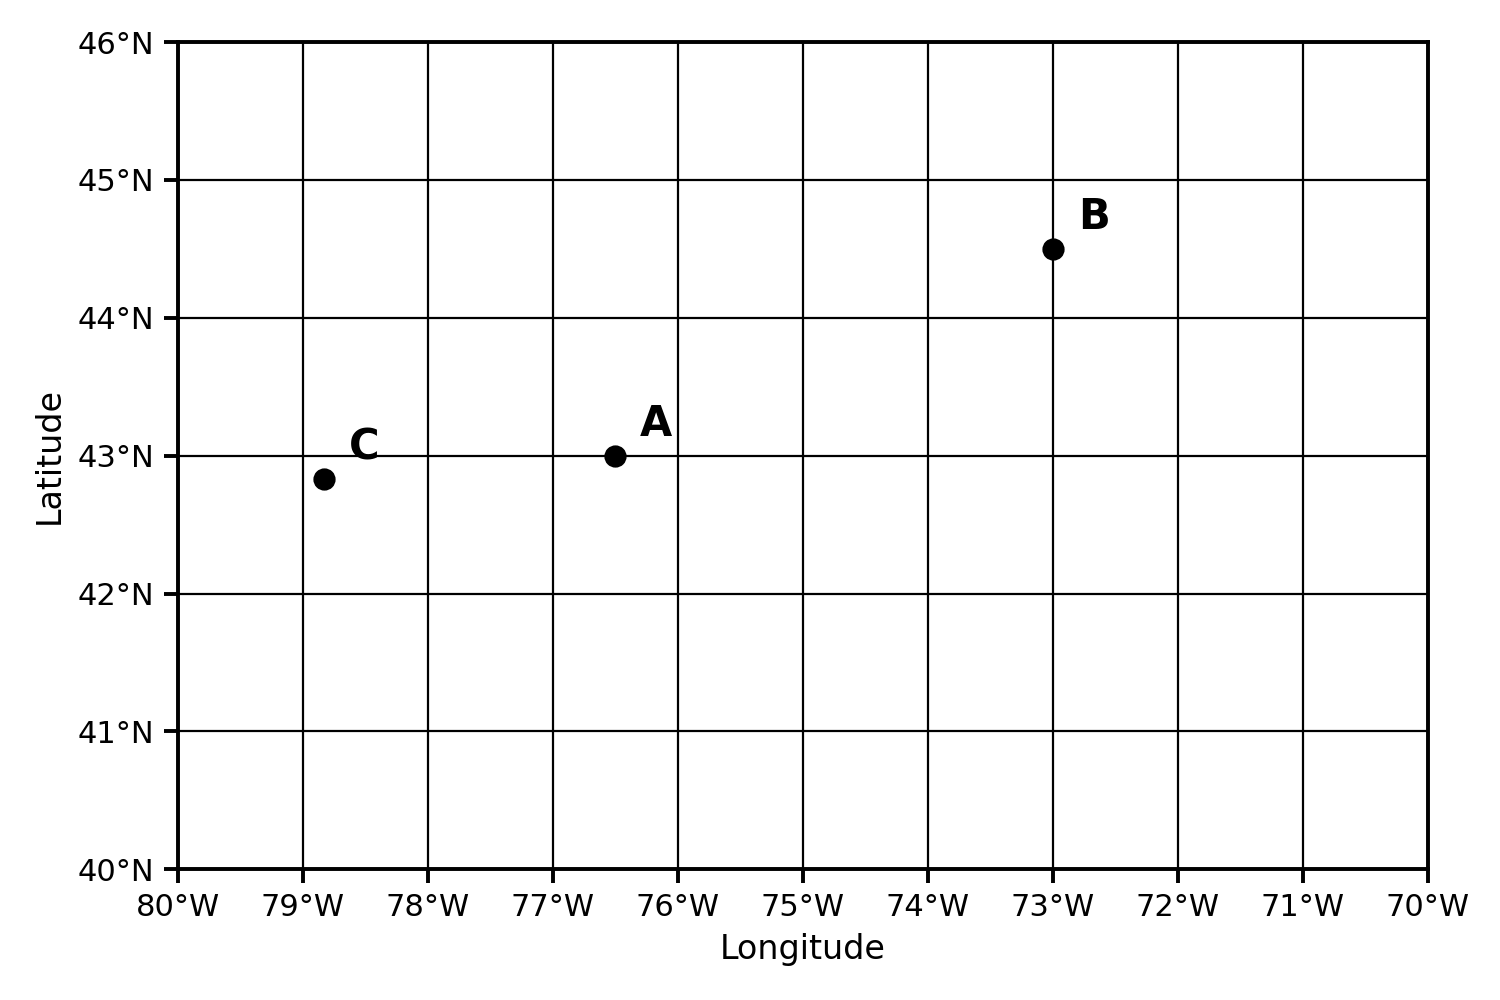
\includegraphics[width=0.78\linewidth]{grid-practice.png}
\end{center}

\vspace{-0.2\baselineskip}
\noindent\begin{tabular}{@{}p{0.5in}p{2.0in}p{2.0in}@{}}
 & \textbf{Latitude} & \textbf{Longitude} \\[2pt]
\textbf{A} & \midblank{43\dg00\mn\ N} & \midblank{76\dg30\mn\ W} \\[6pt]
\textbf{B} & \midblank{44\dg30\mn\ N} & \midblank{73\dg00\mn\ W} \\[6pt]
\textbf{C} & \midblank{42\dg50\mn\ N} & \midblank{78\dg50\mn\ W} \\
\end{tabular}

% ================================================================
\sectiontitle{5. Latitude and Polaris}

\noindent\begin{minipage}[t]{0.50\linewidth}
\vspace{0pt}
Polaris --- the \textbf{North Star} --- sits almost directly above Earth's
\blank{axis of rotation}.

\vspace{0.4\baselineskip}
Because of that, the \textbf{altitude} of Polaris (its angle above the horizon)
is equal to the observer's \blank{latitude}.

\vspace{0.4\baselineskip}
Polaris can only be seen from the \blank{Northern} Hemisphere.
\end{minipage}%
\hfill
\begin{minipage}[t]{0.47\linewidth}
\vspace{0pt}
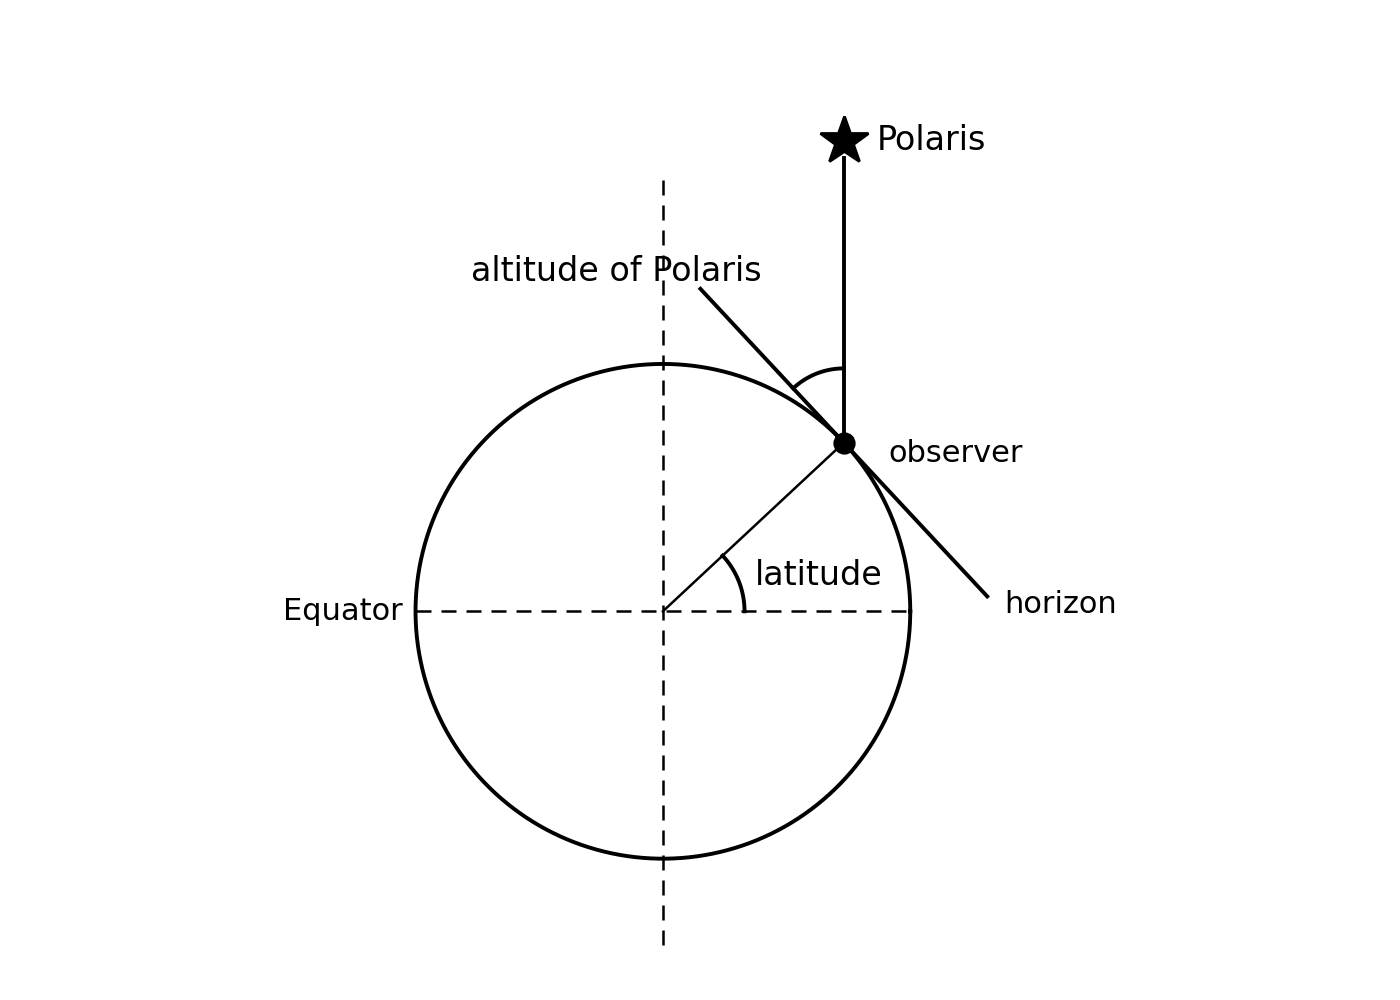
\includegraphics[width=\linewidth]{polaris-latitude.png}
\end{minipage}

\vspace{0.4\baselineskip}
\noindent\textbf{Check the extremes.} Fill in the altitude of Polaris at each location.

\vspace{0.2\baselineskip}
\noindent\begin{tabular}{@{}p{2.3in}p{1.6in}p{2.2in}@{}}
\hline
\textbf{Where you are} & \textbf{Latitude} & \textbf{Altitude of Polaris} \\
\hline
North Pole & 90\dg\ N & \tblblank{90\dg, overhead} \\[4pt]
Albany, NY & 42\dg\ N & \tblblank{42\dg} \\[4pt]
Equator & 0\dg & \tblblank{0\dg, on horizon} \\[4pt]
Southern Hemisphere & --- & \tblblank{not visible} \\
\hline
\end{tabular}

\vspace{0.5\baselineskip}
\noindent\textbf{Moving around.} Circle or fill in what happens to the altitude of Polaris.

\begin{itemize}[nosep,leftmargin=1.6em,itemsep=4pt]
  \item Travel \textbf{north}: Polaris gets \midblank{higher} and latitude \midblank{increases}.
  \item Travel \textbf{south}: Polaris gets \midblank{lower} and latitude \midblank{decreases}.
  \item Travel \textbf{east or west}: Polaris \midblank{does not change} and latitude \midblank{stays the same}.
\end{itemize}

\begin{keyidea}
Moving 1\dg\ of latitude changes the altitude of Polaris by exactly 1\dg\ ---
about 111 km (69 miles) of travel on the ground.
\end{keyidea}

% ================================================================
\sectiontitle{6. Longitude and time zones}

Meridians are counted east and west of the prime meridian until they meet at
\shortblank{180}\dg, which is called the \blank{Int'l Date Line}.

\[ \frac{360\dg \text{ of rotation}}{24 \text{ hours}} = \shortblank{15}\dg \text{ per hour} \]

\begin{keyidea}
Time zones are \shortblank{15}\dg\ of longitude wide, and each one represents
\midblank{1 hour} of time.
\end{keyidea}

\vspace{0.3\baselineskip}
\noindent Earth rotates from west to east, so places to the \textbf{east} rotate into
sunlight first and their clocks are \shortblank{ahead}. Places to the \textbf{west}
have clocks that are \shortblank{behind}.

\vspace{0.4\baselineskip}
\noindent\textbf{Worked example.} Albany is 74\dg\ W. Denver is 105\dg\ W.
How many hours apart are their clocks, and which is earlier?

\vspace{0.2\baselineskip}
\[ 105\dg - 74\dg = \shortblank{31\dg} \qquad \frac{31\dg}{15\dg/\text{h}} \approx \midblank{2 hours} \]

\noindent Denver is \textit{west} of Albany, so Denver's clock is
\blank{2 hours behind}.

% ================================================================
\sectiontitle{7. Check for understanding}

\begin{questions}

\question[1] The angle from the horizon to Polaris is equal to the \rule{0.9in}{0.4pt}
of the observer.
\begin{choices}
  \CorrectChoice latitude
  \choice longitude
\end{choices}

\question[1] Meridians are 15\dg\ apart, so time zones are separated by
\begin{choices}
  \choice 4 hours
  \choice 24 hours
  \CorrectChoice 1 hour
\end{choices}

\question[1] A ship sails due east across the Atlantic Ocean. The altitude of
Polaris will
\begin{choices}
  \choice increase
  \choice decrease
  \CorrectChoice stay the same
\end{choices}

\question[1] How many minutes are in 1\dg\ of latitude?
\begin{choices}
  \choice 10
  \CorrectChoice 60
  \choice 100
\end{choices}

\end{questions}

% ================================================================
\sectiontitle{Exit ticket}

\begin{questions}

\question[2] Using the \textit{Generalized Bedrock Geology of New York State} map in
your ESRT, give the latitude and longitude of Albany, NY to the nearest 10 minutes.

\begin{solutionorbox}[0.55in]
Approximately 42\dg40\mn\ N, 73\dg45\mn\ W.
\end{solutionorbox}

\question[2] An observer measures the altitude of Polaris as 30\dg. What is their
latitude, and which hemisphere are they in? Explain how you know the hemisphere.

\begin{solutionorbox}[0.85in]
They are at 30\dg\ N, in the Northern Hemisphere. Polaris cannot be seen at all
from the Southern Hemisphere, so any observer who can measure its altitude must be
north of the equator.
\end{solutionorbox}

\question[2] Explain in one sentence why time zones are 15\dg\ of longitude wide.

\begin{solutionorbox}[0.7in]
Earth rotates 360\dg\ in 24 hours, which works out to 15\dg\ per hour, so each
15\dg\ of longitude corresponds to one hour of time.
\end{solutionorbox}

\end{questions}

% ================================================================
\sectiontitle{Vocabulary}

\noindent\begin{tabular}{@{}p{1.5in}p{4.9in}@{}}
\textbf{Latitude} & angular distance north or south of the equator, 0\dg\ to 90\dg \\
\textbf{Longitude} & angular distance east or west of the prime meridian, 0\dg\ to 180\dg \\
\textbf{Equator} & the 0\dg\ line of latitude, halfway between the poles \\
\textbf{Prime meridian} & the 0\dg\ line of longitude, through Greenwich, England \\
\textbf{Parallel} & another name for a line of latitude \\
\textbf{Meridian} & another name for a line of longitude \\
\textbf{Altitude} & the angle of an object above the horizon \\
\textbf{Int'l Date Line} & the 180\dg\ meridian, where the calendar date changes \\
\end{tabular}

\end{document}
"

\documentclass[11pt,addpoints]{exam}

\usepackage[margin=0.85in,top=1.1in,headsep=0.25in]{geometry}
\usepackage{graphicx}
\usepackage{amsmath}
\usepackage{textcomp}
\usepackage{enumitem}
\usepackage{xcolor}
\usepackage{tcolorbox}
\usepackage{parskip}
\usepackage{needspace}

\ifdefined\answerkey
  \printanswers
\fi

% ---------------------------------------------------------------- formatting
\pagestyle{headandfoot}
\firstpageheader{\textbf{Earth's Coordinates}}{}{Name: \makebox[1.6in]{\hrulefill}}
\runningheader{\textbf{Earth's Coordinates}}{}{Name: \makebox[1.6in]{\hrulefill}}
\firstpagefooter{Earth Science}{Page \thepage\ of \numpages}{Date: \makebox[1.1in]{\hrulefill}\ \ Per: \makebox[0.4in]{\hrulefill}}
\runningfooter{Earth Science}{Page \thepage\ of \numpages}{}
\headrule
\footrule

\renewcommand{\thequestion}{\arabic{question}}
\pointsinrightmargin
\bracketedpoints

\newcommand{\dg}{\ensuremath{^{\circ}}}
\newcommand{\mn}{\ensuremath{'}}

% a fill-in blank of standard width
\newcommand{\blank}[1]{\fillin[#1][1.35in]}
\newcommand{\shortblank}[1]{\fillin[#1][0.85in]}
\newcommand{\longblank}[1]{\fillin[#1][2.6in]}
\newcommand{\tblblank}[1]{\fillin[#1][1.2in]}
\newcommand{\midblank}[1]{\fillin[#1][1.1in]}

% open-response prompt: ruled lines for students, answer text for the key
\newcounter{rl}
\newcommand{\responselines}[1]{%
  \setcounter{rl}{0}%
  \loop\ifnum\value{rl}<#1\relax
    \noindent\rule{\linewidth}{0.4pt}\par\vspace{1.15\baselineskip}%
    \stepcounter{rl}%
  \repeat}
\newcommand{\openresponse}[2][2]{%
  \ifdefined\answerkey
    \par\vspace{0.2\baselineskip}\noindent\textbf{#2}\par\vspace{0.4\baselineskip}%
  \else
    \par\vspace{0.6\baselineskip}\responselines{#1}%
  \fi}

\newtcolorbox{keyidea}{
  colback=black!4, colframe=black!55, boxrule=0.6pt,
  left=6pt, right=6pt, top=5pt, bottom=5pt, arc=2pt
}

\newcommand{\sectiontitle}[1]{%
  \needspace{6\baselineskip}%
  \vspace{0.6\baselineskip}%
  \noindent\textbf{\large #1}\par\nopagebreak
  \vspace{-0.4\baselineskip}\noindent\rule{\linewidth}{0.8pt}\par\nopagebreak
  \vspace{0.2\baselineskip}}

% ---------------------------------------------------------------- document
\begin{document}

\begin{center}
  {\Large\textbf{Earth's Coordinates}}\\[2pt]
  {\large Guided Notes \ifdefined\answerkey\textbf{--- ANSWER KEY}\fi}\\[4pt]
  \textit{Driving question: How do we locate things on Earth?}
\end{center}

\vspace{0.4\baselineskip}

% ================================================================
\sectiontitle{1. Why we need a coordinate system}

Directions given by landmark (``two miles past the old barn'') only work if you
already know the landmark. A \textbf{coordinate system} gives every point on Earth
one unique address built from a grid of \blank{intersecting} lines.

\begin{keyidea}
The grid is anchored to something that never moves: Earth's \blank{axis of rotation}.
The poles and the equator come from the way Earth spins, not from a human decision.
\end{keyidea}

% ================================================================
\sectiontitle{2. Latitude and longitude}

Complete the table.

\vspace{0.3\baselineskip}
\renewcommand{\arraystretch}{1.9}
\noindent\begin{tabular}{@{}p{1.5in}p{2.4in}p{2.4in}@{}}
\hline
 & \textbf{Latitude} & \textbf{Longitude} \\
\hline
Lines run\dots & \tblblank{east--west} & \tblblank{north--south} \\
Measured\dots & \tblblank{north--south} & \tblblank{east--west} \\
Do they touch? & \tblblank{no, parallel} & \tblblank{yes, at the poles} \\
Measured from\dots & \tblblank{the equator} & \tblblank{prime meridian} \\
That line is\dots & 0\dg\ latitude & 0\dg\ longitude \\
Range & 0\dg\ to \shortblank{90\dg} N or S & 0\dg\ to \shortblank{180\dg} E or W \\
\hline
\end{tabular}
\renewcommand{\arraystretch}{1}

\vspace{0.5\baselineskip}

\begin{keyidea}
Every coordinate needs \textbf{a number AND a direction}. 43\dg\ is not a location.
43\dg\ N is a line; 43\dg\ N, 76\dg\ W is a point.\\[3pt]
\textbf{Latitude is always written first.}
\end{keyidea}

\vspace{0.3\baselineskip}
\noindent Why does latitude stop at 90\dg\ but longitude go to 180\dg?

\openresponse[2]{At 90\dg\ you have reached the pole --- there is no more Earth to travel.
Longitude can run 180\dg\ each way because you can circle halfway around in either direction.}

% ================================================================
\sectiontitle{3. Degrees and minutes}

When we zoom in, latitude and longitude are given in degrees \textit{and}
\textbf{minutes}, written with a prime symbol (\mn).

\[ 1\dg = \shortblank{60}\mn \qquad 30\mn = \tfrac{1}{2}\dg \qquad 10\mn = \tfrac{1}{6}\dg \]

\begin{itemize}[nosep,leftmargin=1.6em]
  \item Halfway between two degree lines is about \shortblank{30}\mn.
  \item We estimate minutes to the nearest \shortblank{10} minutes.
\end{itemize}

\vspace{0.3\baselineskip}
\noindent\textbf{Watch out:} 76.5\dg\ is \textbf{not} 76\dg50\mn. Half a degree is
\shortblank{30}\mn, just like half an hour is 30 minutes.

\vspace{0.3\baselineskip}
\noindent\textbf{Worked example.} Syracuse, NY sits on the 43\dg\ parallel and a
little past the 76\dg\ meridian:\quad \blank{43\dg\ N, 76\dg10\mn\ W}

% ================================================================
\sectiontitle{4. Practice: reading the grid}

Give the latitude and longitude of each point to the nearest 10 minutes.
Remember the hemisphere letters.

\begin{center}
  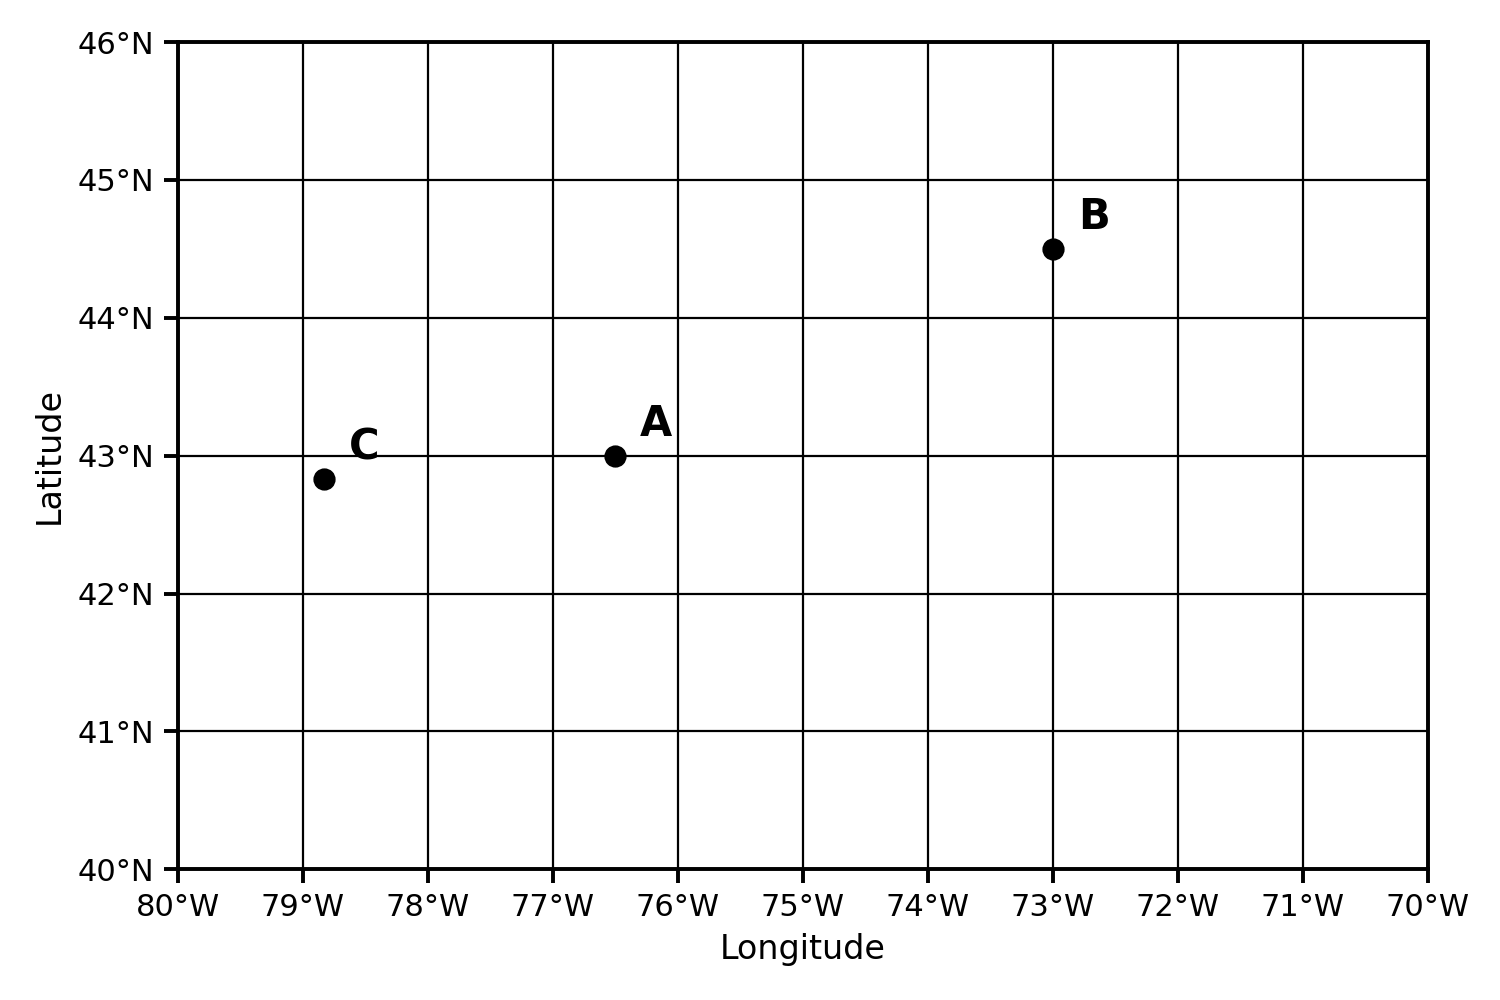
\includegraphics[width=0.78\linewidth]{grid-practice.png}
\end{center}

\vspace{-0.2\baselineskip}
\noindent\begin{tabular}{@{}p{0.5in}p{2.0in}p{2.0in}@{}}
 & \textbf{Latitude} & \textbf{Longitude} \\[2pt]
\textbf{A} & \midblank{43\dg00\mn\ N} & \midblank{76\dg30\mn\ W} \\[6pt]
\textbf{B} & \midblank{44\dg30\mn\ N} & \midblank{73\dg00\mn\ W} \\[6pt]
\textbf{C} & \midblank{42\dg50\mn\ N} & \midblank{78\dg50\mn\ W} \\
\end{tabular}

% ================================================================
\sectiontitle{5. Latitude and Polaris}

\noindent\begin{minipage}[t]{0.50\linewidth}
\vspace{0pt}
Polaris --- the \textbf{North Star} --- sits almost directly above Earth's
\blank{axis of rotation}.

\vspace{0.4\baselineskip}
Because of that, the \textbf{altitude} of Polaris (its angle above the horizon)
is equal to the observer's \blank{latitude}.

\vspace{0.4\baselineskip}
Polaris can only be seen from the \blank{Northern} Hemisphere.
\end{minipage}%
\hfill
\begin{minipage}[t]{0.47\linewidth}
\vspace{0pt}
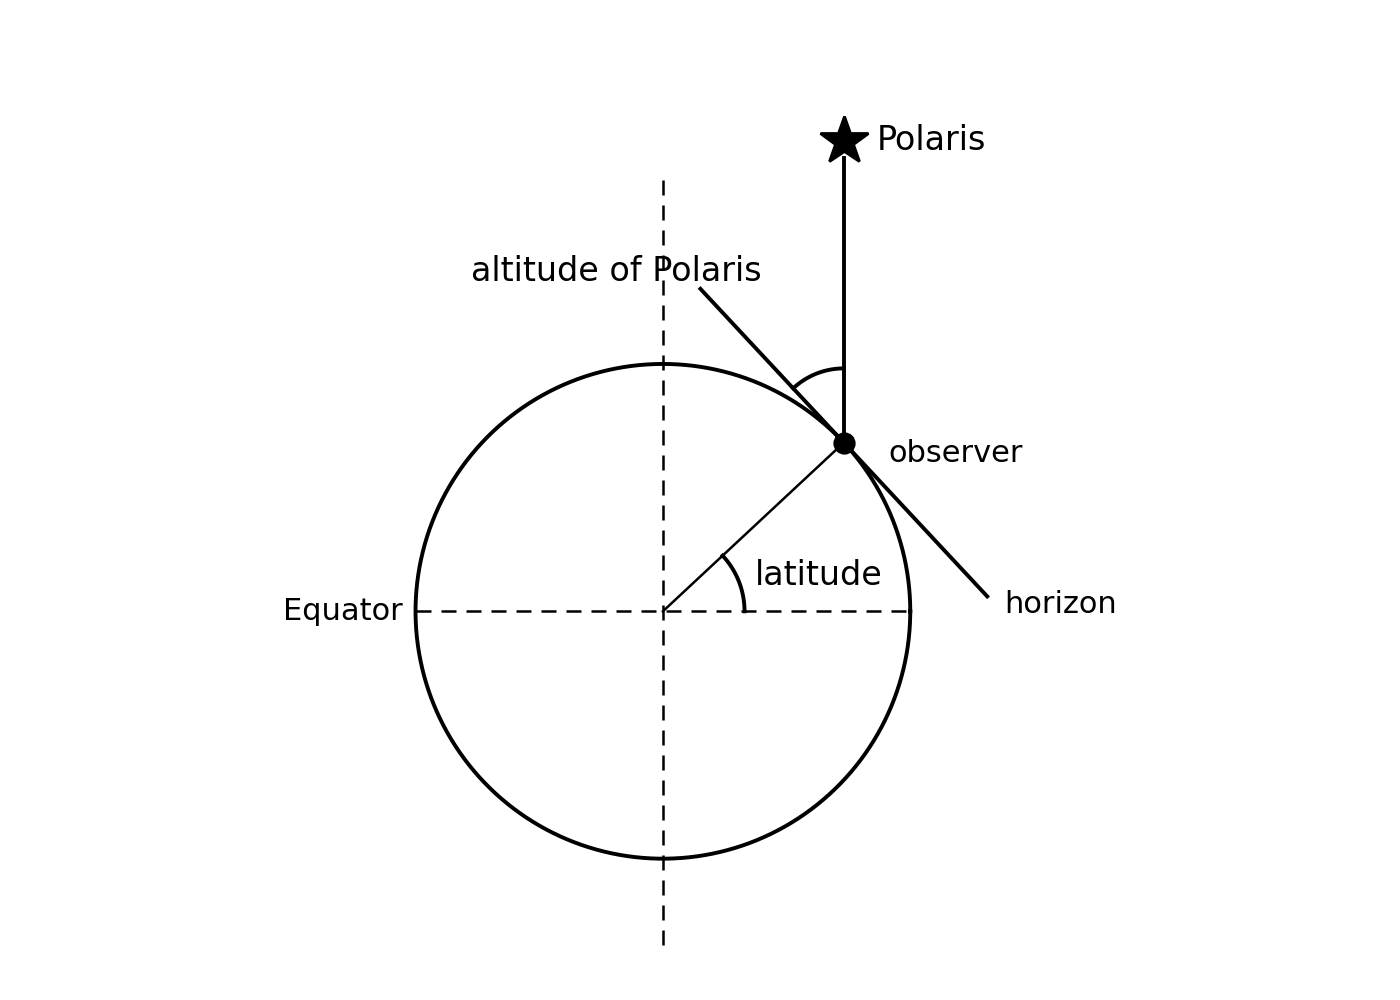
\includegraphics[width=\linewidth]{polaris-latitude.png}
\end{minipage}

\vspace{0.4\baselineskip}
\noindent\textbf{Check the extremes.} Fill in the altitude of Polaris at each location.

\vspace{0.2\baselineskip}
\noindent\begin{tabular}{@{}p{2.3in}p{1.6in}p{2.2in}@{}}
\hline
\textbf{Where you are} & \textbf{Latitude} & \textbf{Altitude of Polaris} \\
\hline
North Pole & 90\dg\ N & \tblblank{90\dg, overhead} \\[4pt]
Albany, NY & 42\dg\ N & \tblblank{42\dg} \\[4pt]
Equator & 0\dg & \tblblank{0\dg, on horizon} \\[4pt]
Southern Hemisphere & --- & \tblblank{not visible} \\
\hline
\end{tabular}

\vspace{0.5\baselineskip}
\noindent\textbf{Moving around.} Circle or fill in what happens to the altitude of Polaris.

\begin{itemize}[nosep,leftmargin=1.6em,itemsep=4pt]
  \item Travel \textbf{north}: Polaris gets \midblank{higher} and latitude \midblank{increases}.
  \item Travel \textbf{south}: Polaris gets \midblank{lower} and latitude \midblank{decreases}.
  \item Travel \textbf{east or west}: Polaris \midblank{does not change} and latitude \midblank{stays the same}.
\end{itemize}

\begin{keyidea}
Moving 1\dg\ of latitude changes the altitude of Polaris by exactly 1\dg\ ---
about 111 km (69 miles) of travel on the ground.
\end{keyidea}

% ================================================================
\sectiontitle{6. Longitude and time zones}

Meridians are counted east and west of the prime meridian until they meet at
\shortblank{180}\dg, which is called the \blank{Int'l Date Line}.

\[ \frac{360\dg \text{ of rotation}}{24 \text{ hours}} = \shortblank{15}\dg \text{ per hour} \]

\begin{keyidea}
Time zones are \shortblank{15}\dg\ of longitude wide, and each one represents
\midblank{1 hour} of time.
\end{keyidea}

\vspace{0.3\baselineskip}
\noindent Earth rotates from west to east, so places to the \textbf{east} rotate into
sunlight first and their clocks are \shortblank{ahead}. Places to the \textbf{west}
have clocks that are \shortblank{behind}.

\vspace{0.4\baselineskip}
\noindent\textbf{Worked example.} Albany is 74\dg\ W. Denver is 105\dg\ W.
How many hours apart are their clocks, and which is earlier?

\vspace{0.2\baselineskip}
\[ 105\dg - 74\dg = \shortblank{31\dg} \qquad \frac{31\dg}{15\dg/\text{h}} \approx \midblank{2 hours} \]

\noindent Denver is \textit{west} of Albany, so Denver's clock is
\blank{2 hours behind}.

% ================================================================
\sectiontitle{7. Check for understanding}

\begin{questions}

\question[1] The angle from the horizon to Polaris is equal to the \rule{0.9in}{0.4pt}
of the observer.
\begin{choices}
  \CorrectChoice latitude
  \choice longitude
\end{choices}

\question[1] Meridians are 15\dg\ apart, so time zones are separated by
\begin{choices}
  \choice 4 hours
  \choice 24 hours
  \CorrectChoice 1 hour
\end{choices}

\question[1] A ship sails due east across the Atlantic Ocean. The altitude of
Polaris will
\begin{choices}
  \choice increase
  \choice decrease
  \CorrectChoice stay the same
\end{choices}

\question[1] How many minutes are in 1\dg\ of latitude?
\begin{choices}
  \choice 10
  \CorrectChoice 60
  \choice 100
\end{choices}

\end{questions}

% ================================================================
\sectiontitle{Exit ticket}

\begin{questions}

\question[2] Using the \textit{Generalized Bedrock Geology of New York State} map in
your ESRT, give the latitude and longitude of Albany, NY to the nearest 10 minutes.

\begin{solutionorbox}[0.55in]
Approximately 42\dg40\mn\ N, 73\dg45\mn\ W.
\end{solutionorbox}

\question[2] An observer measures the altitude of Polaris as 30\dg. What is their
latitude, and which hemisphere are they in? Explain how you know the hemisphere.

\begin{solutionorbox}[0.85in]
They are at 30\dg\ N, in the Northern Hemisphere. Polaris cannot be seen at all
from the Southern Hemisphere, so any observer who can measure its altitude must be
north of the equator.
\end{solutionorbox}

\question[2] Explain in one sentence why time zones are 15\dg\ of longitude wide.

\begin{solutionorbox}[0.7in]
Earth rotates 360\dg\ in 24 hours, which works out to 15\dg\ per hour, so each
15\dg\ of longitude corresponds to one hour of time.
\end{solutionorbox}

\end{questions}

% ================================================================
\sectiontitle{Vocabulary}

\noindent\begin{tabular}{@{}p{1.5in}p{4.9in}@{}}
\textbf{Latitude} & angular distance north or south of the equator, 0\dg\ to 90\dg \\
\textbf{Longitude} & angular distance east or west of the prime meridian, 0\dg\ to 180\dg \\
\textbf{Equator} & the 0\dg\ line of latitude, halfway between the poles \\
\textbf{Prime meridian} & the 0\dg\ line of longitude, through Greenwich, England \\
\textbf{Parallel} & another name for a line of latitude \\
\textbf{Meridian} & another name for a line of longitude \\
\textbf{Altitude} & the angle of an object above the horizon \\
\textbf{Int'l Date Line} & the 180\dg\ meridian, where the calendar date changes \\
\end{tabular}

\end{document}
"

\documentclass[11pt,addpoints]{exam}

\usepackage[margin=0.85in,top=1.1in,headsep=0.25in]{geometry}
\usepackage{graphicx}
\usepackage{amsmath}
\usepackage{textcomp}
\usepackage{enumitem}
\usepackage{xcolor}
\usepackage{tcolorbox}
\usepackage{parskip}
\usepackage{needspace}

\ifdefined\answerkey
  \printanswers
\fi

% ---------------------------------------------------------------- formatting
\pagestyle{headandfoot}
\firstpageheader{\textbf{Earth's Coordinates}}{}{Name: \makebox[1.6in]{\hrulefill}}
\runningheader{\textbf{Earth's Coordinates}}{}{Name: \makebox[1.6in]{\hrulefill}}
\firstpagefooter{Earth Science}{Page \thepage\ of \numpages}{Date: \makebox[1.1in]{\hrulefill}\ \ Per: \makebox[0.4in]{\hrulefill}}
\runningfooter{Earth Science}{Page \thepage\ of \numpages}{}
\headrule
\footrule

\renewcommand{\thequestion}{\arabic{question}}
\pointsinrightmargin
\bracketedpoints

\newcommand{\dg}{\ensuremath{^{\circ}}}
\newcommand{\mn}{\ensuremath{'}}

% a fill-in blank of standard width
\newcommand{\blank}[1]{\fillin[#1][1.35in]}
\newcommand{\shortblank}[1]{\fillin[#1][0.85in]}
\newcommand{\longblank}[1]{\fillin[#1][2.6in]}
\newcommand{\tblblank}[1]{\fillin[#1][1.2in]}
\newcommand{\midblank}[1]{\fillin[#1][1.1in]}

% open-response prompt: ruled lines for students, answer text for the key
\newcounter{rl}
\newcommand{\responselines}[1]{%
  \setcounter{rl}{0}%
  \loop\ifnum\value{rl}<#1\relax
    \noindent\rule{\linewidth}{0.4pt}\par\vspace{1.15\baselineskip}%
    \stepcounter{rl}%
  \repeat}
\newcommand{\openresponse}[2][2]{%
  \ifdefined\answerkey
    \par\vspace{0.2\baselineskip}\noindent\textbf{#2}\par\vspace{0.4\baselineskip}%
  \else
    \par\vspace{0.6\baselineskip}\responselines{#1}%
  \fi}

\newtcolorbox{keyidea}{
  colback=black!4, colframe=black!55, boxrule=0.6pt,
  left=6pt, right=6pt, top=5pt, bottom=5pt, arc=2pt
}

\newcommand{\sectiontitle}[1]{%
  \needspace{6\baselineskip}%
  \vspace{0.6\baselineskip}%
  \noindent\textbf{\large #1}\par\nopagebreak
  \vspace{-0.4\baselineskip}\noindent\rule{\linewidth}{0.8pt}\par\nopagebreak
  \vspace{0.2\baselineskip}}

% ---------------------------------------------------------------- document
\begin{document}

\begin{center}
  {\Large\textbf{Earth's Coordinates}}\\[2pt]
  {\large Guided Notes \ifdefined\answerkey\textbf{--- ANSWER KEY}\fi}\\[4pt]
  \textit{Driving question: How do we locate things on Earth?}
\end{center}

\vspace{0.4\baselineskip}

% ================================================================
\sectiontitle{1. Why we need a coordinate system}

Directions given by landmark (``two miles past the old barn'') only work if you
already know the landmark. A \textbf{coordinate system} gives every point on Earth
one unique address built from a grid of \blank{intersecting} lines.

\begin{keyidea}
The grid is anchored to something that never moves: Earth's \blank{axis of rotation}.
The poles and the equator come from the way Earth spins, not from a human decision.
\end{keyidea}

% ================================================================
\sectiontitle{2. Latitude and longitude}

Complete the table.

\vspace{0.3\baselineskip}
\renewcommand{\arraystretch}{1.9}
\noindent\begin{tabular}{@{}p{1.5in}p{2.4in}p{2.4in}@{}}
\hline
 & \textbf{Latitude} & \textbf{Longitude} \\
\hline
Lines run\dots & \tblblank{east--west} & \tblblank{north--south} \\
Measured\dots & \tblblank{north--south} & \tblblank{east--west} \\
Do they touch? & \tblblank{no, parallel} & \tblblank{yes, at the poles} \\
Measured from\dots & \tblblank{the equator} & \tblblank{prime meridian} \\
That line is\dots & 0\dg\ latitude & 0\dg\ longitude \\
Range & 0\dg\ to \shortblank{90\dg} N or S & 0\dg\ to \shortblank{180\dg} E or W \\
\hline
\end{tabular}
\renewcommand{\arraystretch}{1}

\vspace{0.5\baselineskip}

\begin{keyidea}
Every coordinate needs \textbf{a number AND a direction}. 43\dg\ is not a location.
43\dg\ N is a line; 43\dg\ N, 76\dg\ W is a point.\\[3pt]
\textbf{Latitude is always written first.}
\end{keyidea}

\vspace{0.3\baselineskip}
\noindent Why does latitude stop at 90\dg\ but longitude go to 180\dg?

\openresponse[2]{At 90\dg\ you have reached the pole --- there is no more Earth to travel.
Longitude can run 180\dg\ each way because you can circle halfway around in either direction.}

% ================================================================
\sectiontitle{3. Degrees and minutes}

When we zoom in, latitude and longitude are given in degrees \textit{and}
\textbf{minutes}, written with a prime symbol (\mn).

\[ 1\dg = \shortblank{60}\mn \qquad 30\mn = \tfrac{1}{2}\dg \qquad 10\mn = \tfrac{1}{6}\dg \]

\begin{itemize}[nosep,leftmargin=1.6em]
  \item Halfway between two degree lines is about \shortblank{30}\mn.
  \item We estimate minutes to the nearest \shortblank{10} minutes.
\end{itemize}

\vspace{0.3\baselineskip}
\noindent\textbf{Watch out:} 76.5\dg\ is \textbf{not} 76\dg50\mn. Half a degree is
\shortblank{30}\mn, just like half an hour is 30 minutes.

\vspace{0.3\baselineskip}
\noindent\textbf{Worked example.} Syracuse, NY sits on the 43\dg\ parallel and a
little past the 76\dg\ meridian:\quad \blank{43\dg\ N, 76\dg10\mn\ W}

% ================================================================
\sectiontitle{4. Practice: reading the grid}

Give the latitude and longitude of each point to the nearest 10 minutes.
Remember the hemisphere letters.

\begin{center}
  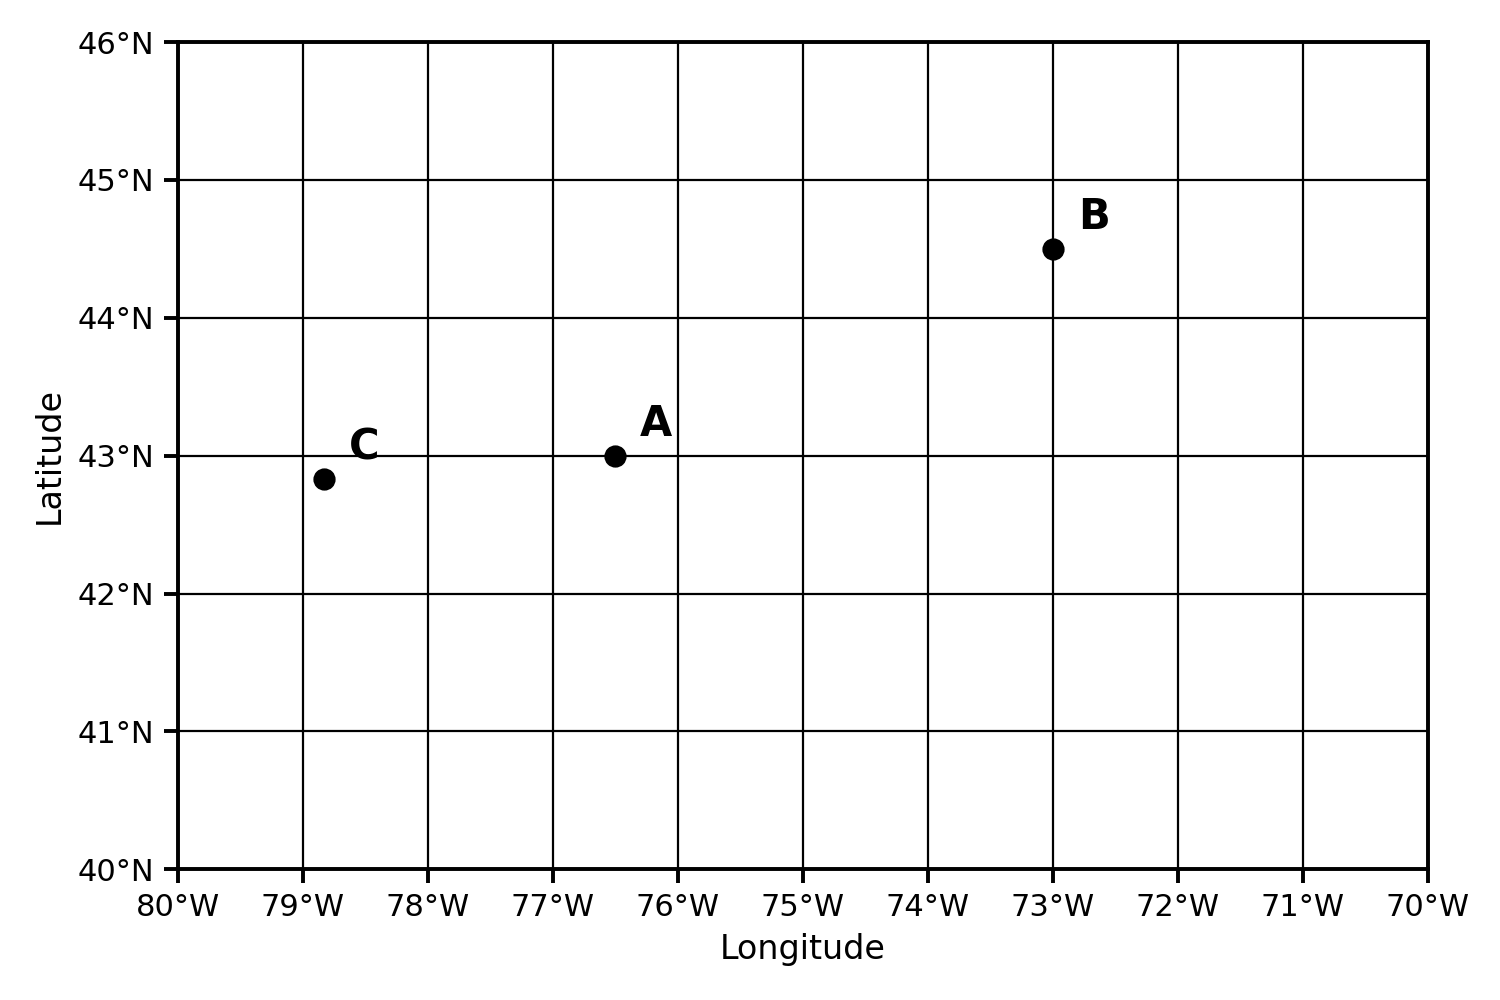
\includegraphics[width=0.78\linewidth]{grid-practice.png}
\end{center}

\vspace{-0.2\baselineskip}
\noindent\begin{tabular}{@{}p{0.5in}p{2.0in}p{2.0in}@{}}
 & \textbf{Latitude} & \textbf{Longitude} \\[2pt]
\textbf{A} & \midblank{43\dg00\mn\ N} & \midblank{76\dg30\mn\ W} \\[6pt]
\textbf{B} & \midblank{44\dg30\mn\ N} & \midblank{73\dg00\mn\ W} \\[6pt]
\textbf{C} & \midblank{42\dg50\mn\ N} & \midblank{78\dg50\mn\ W} \\
\end{tabular}

% ================================================================
\sectiontitle{5. Latitude and Polaris}

\noindent\begin{minipage}[t]{0.50\linewidth}
\vspace{0pt}
Polaris --- the \textbf{North Star} --- sits almost directly above Earth's
\blank{axis of rotation}.

\vspace{0.4\baselineskip}
Because of that, the \textbf{altitude} of Polaris (its angle above the horizon)
is equal to the observer's \blank{latitude}.

\vspace{0.4\baselineskip}
Polaris can only be seen from the \blank{Northern} Hemisphere.
\end{minipage}%
\hfill
\begin{minipage}[t]{0.47\linewidth}
\vspace{0pt}
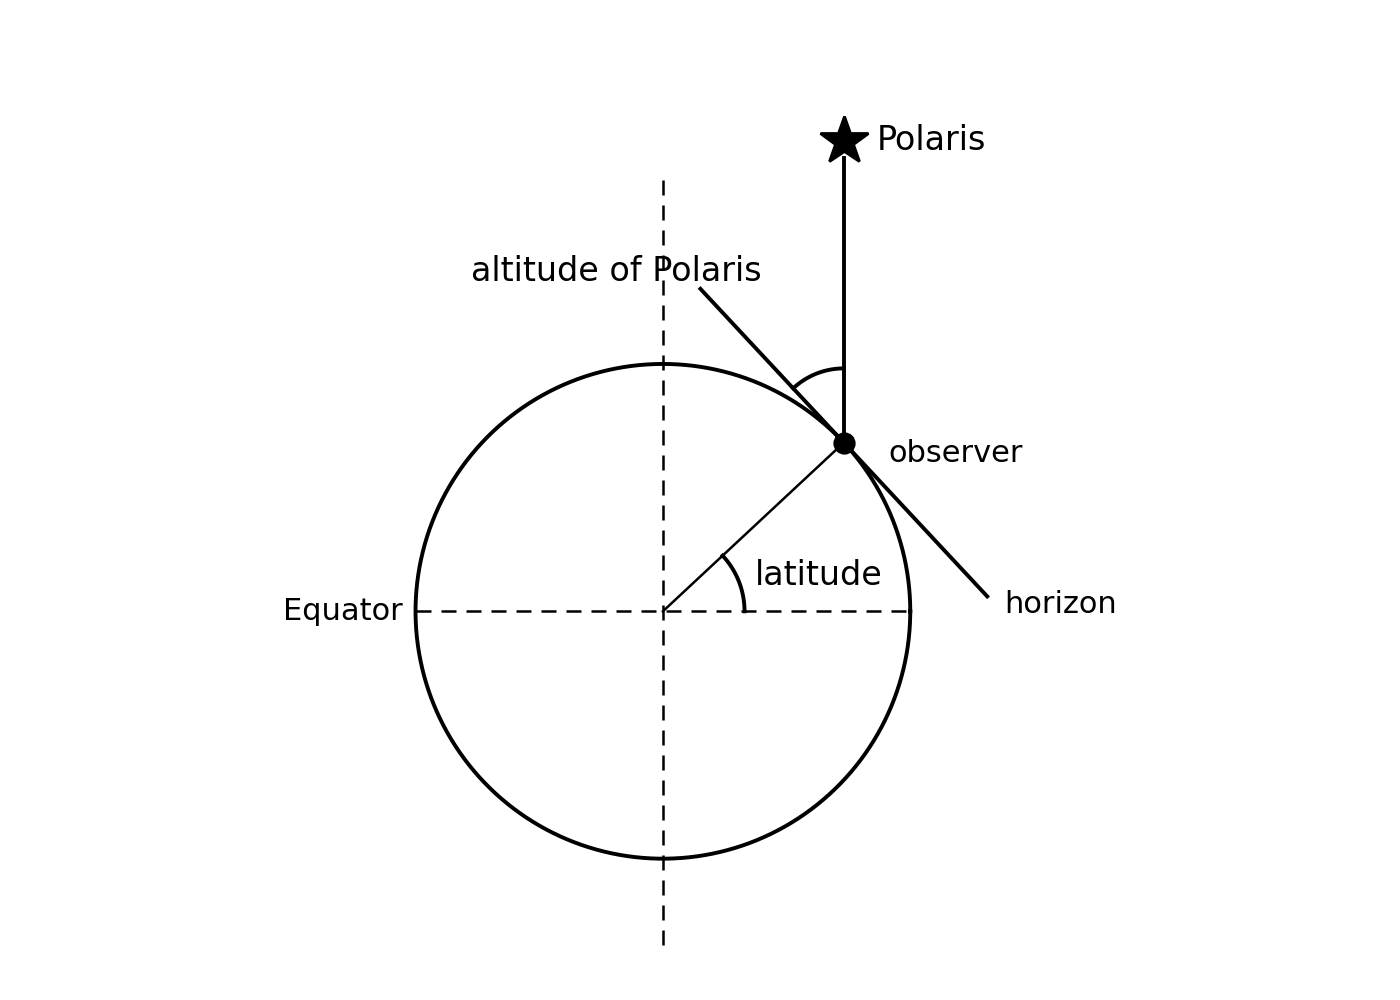
\includegraphics[width=\linewidth]{polaris-latitude.png}
\end{minipage}

\vspace{0.4\baselineskip}
\noindent\textbf{Check the extremes.} Fill in the altitude of Polaris at each location.

\vspace{0.2\baselineskip}
\noindent\begin{tabular}{@{}p{2.3in}p{1.6in}p{2.2in}@{}}
\hline
\textbf{Where you are} & \textbf{Latitude} & \textbf{Altitude of Polaris} \\
\hline
North Pole & 90\dg\ N & \tblblank{90\dg, overhead} \\[4pt]
Albany, NY & 42\dg\ N & \tblblank{42\dg} \\[4pt]
Equator & 0\dg & \tblblank{0\dg, on horizon} \\[4pt]
Southern Hemisphere & --- & \tblblank{not visible} \\
\hline
\end{tabular}

\vspace{0.5\baselineskip}
\noindent\textbf{Moving around.} Circle or fill in what happens to the altitude of Polaris.

\begin{itemize}[nosep,leftmargin=1.6em,itemsep=4pt]
  \item Travel \textbf{north}: Polaris gets \midblank{higher} and latitude \midblank{increases}.
  \item Travel \textbf{south}: Polaris gets \midblank{lower} and latitude \midblank{decreases}.
  \item Travel \textbf{east or west}: Polaris \midblank{does not change} and latitude \midblank{stays the same}.
\end{itemize}

\begin{keyidea}
Moving 1\dg\ of latitude changes the altitude of Polaris by exactly 1\dg\ ---
about 111 km (69 miles) of travel on the ground.
\end{keyidea}

% ================================================================
\sectiontitle{6. Longitude and time zones}

Meridians are counted east and west of the prime meridian until they meet at
\shortblank{180}\dg, which is called the \blank{Int'l Date Line}.

\[ \frac{360\dg \text{ of rotation}}{24 \text{ hours}} = \shortblank{15}\dg \text{ per hour} \]

\begin{keyidea}
Time zones are \shortblank{15}\dg\ of longitude wide, and each one represents
\midblank{1 hour} of time.
\end{keyidea}

\vspace{0.3\baselineskip}
\noindent Earth rotates from west to east, so places to the \textbf{east} rotate into
sunlight first and their clocks are \shortblank{ahead}. Places to the \textbf{west}
have clocks that are \shortblank{behind}.

\vspace{0.4\baselineskip}
\noindent\textbf{Worked example.} Albany is 74\dg\ W. Denver is 105\dg\ W.
How many hours apart are their clocks, and which is earlier?

\vspace{0.2\baselineskip}
\[ 105\dg - 74\dg = \shortblank{31\dg} \qquad \frac{31\dg}{15\dg/\text{h}} \approx \midblank{2 hours} \]

\noindent Denver is \textit{west} of Albany, so Denver's clock is
\blank{2 hours behind}.

% ================================================================
\sectiontitle{7. Check for understanding}

\begin{questions}

\question[1] The angle from the horizon to Polaris is equal to the \rule{0.9in}{0.4pt}
of the observer.
\begin{choices}
  \CorrectChoice latitude
  \choice longitude
\end{choices}

\question[1] Meridians are 15\dg\ apart, so time zones are separated by
\begin{choices}
  \choice 4 hours
  \choice 24 hours
  \CorrectChoice 1 hour
\end{choices}

\question[1] A ship sails due east across the Atlantic Ocean. The altitude of
Polaris will
\begin{choices}
  \choice increase
  \choice decrease
  \CorrectChoice stay the same
\end{choices}

\question[1] How many minutes are in 1\dg\ of latitude?
\begin{choices}
  \choice 10
  \CorrectChoice 60
  \choice 100
\end{choices}

\end{questions}

% ================================================================
\sectiontitle{Exit ticket}

\begin{questions}

\question[2] Using the \textit{Generalized Bedrock Geology of New York State} map in
your ESRT, give the latitude and longitude of Albany, NY to the nearest 10 minutes.

\begin{solutionorbox}[0.55in]
Approximately 42\dg40\mn\ N, 73\dg45\mn\ W.
\end{solutionorbox}

\question[2] An observer measures the altitude of Polaris as 30\dg. What is their
latitude, and which hemisphere are they in? Explain how you know the hemisphere.

\begin{solutionorbox}[0.85in]
They are at 30\dg\ N, in the Northern Hemisphere. Polaris cannot be seen at all
from the Southern Hemisphere, so any observer who can measure its altitude must be
north of the equator.
\end{solutionorbox}

\question[2] Explain in one sentence why time zones are 15\dg\ of longitude wide.

\begin{solutionorbox}[0.7in]
Earth rotates 360\dg\ in 24 hours, which works out to 15\dg\ per hour, so each
15\dg\ of longitude corresponds to one hour of time.
\end{solutionorbox}

\end{questions}

% ================================================================
\sectiontitle{Vocabulary}

\noindent\begin{tabular}{@{}p{1.5in}p{4.9in}@{}}
\textbf{Latitude} & angular distance north or south of the equator, 0\dg\ to 90\dg \\
\textbf{Longitude} & angular distance east or west of the prime meridian, 0\dg\ to 180\dg \\
\textbf{Equator} & the 0\dg\ line of latitude, halfway between the poles \\
\textbf{Prime meridian} & the 0\dg\ line of longitude, through Greenwich, England \\
\textbf{Parallel} & another name for a line of latitude \\
\textbf{Meridian} & another name for a line of longitude \\
\textbf{Altitude} & the angle of an object above the horizon \\
\textbf{Int'l Date Line} & the 180\dg\ meridian, where the calendar date changes \\
\end{tabular}

\end{document}
"

\documentclass[11pt,addpoints]{exam}

\usepackage[margin=0.85in,top=1.1in,headsep=0.25in]{geometry}
\usepackage{graphicx}
\usepackage{amsmath}
\usepackage{textcomp}
\usepackage{enumitem}
\usepackage{xcolor}
\usepackage{tcolorbox}
\usepackage{parskip}
\usepackage{needspace}

\ifdefined\answerkey
  \printanswers
\fi

% ---------------------------------------------------------------- formatting
\pagestyle{headandfoot}
\firstpageheader{\textbf{Earth's Coordinates}}{}{Name: \makebox[1.6in]{\hrulefill}}
\runningheader{\textbf{Earth's Coordinates}}{}{Name: \makebox[1.6in]{\hrulefill}}
\firstpagefooter{Earth Science}{Page \thepage\ of \numpages}{Date: \makebox[1.1in]{\hrulefill}\ \ Per: \makebox[0.4in]{\hrulefill}}
\runningfooter{Earth Science}{Page \thepage\ of \numpages}{}
\headrule
\footrule

\renewcommand{\thequestion}{\arabic{question}}
\pointsinrightmargin
\bracketedpoints

\newcommand{\dg}{\ensuremath{^{\circ}}}
\newcommand{\mn}{\ensuremath{'}}

% a fill-in blank of standard width
\newcommand{\blank}[1]{\fillin[#1][1.35in]}
\newcommand{\shortblank}[1]{\fillin[#1][0.85in]}
\newcommand{\longblank}[1]{\fillin[#1][2.6in]}
\newcommand{\tblblank}[1]{\fillin[#1][1.2in]}
\newcommand{\midblank}[1]{\fillin[#1][1.1in]}

% open-response prompt: ruled lines for students, answer text for the key
\newcounter{rl}
\newcommand{\responselines}[1]{%
  \setcounter{rl}{0}%
  \loop\ifnum\value{rl}<#1\relax
    \noindent\rule{\linewidth}{0.4pt}\par\vspace{1.15\baselineskip}%
    \stepcounter{rl}%
  \repeat}
\newcommand{\openresponse}[2][2]{%
  \ifdefined\answerkey
    \par\vspace{0.2\baselineskip}\noindent\textbf{#2}\par\vspace{0.4\baselineskip}%
  \else
    \par\vspace{0.6\baselineskip}\responselines{#1}%
  \fi}

\newtcolorbox{keyidea}{
  colback=black!4, colframe=black!55, boxrule=0.6pt,
  left=6pt, right=6pt, top=5pt, bottom=5pt, arc=2pt
}

\newcommand{\sectiontitle}[1]{%
  \needspace{6\baselineskip}%
  \vspace{0.6\baselineskip}%
  \noindent\textbf{\large #1}\par\nopagebreak
  \vspace{-0.4\baselineskip}\noindent\rule{\linewidth}{0.8pt}\par\nopagebreak
  \vspace{0.2\baselineskip}}

% ---------------------------------------------------------------- document
\begin{document}

\begin{center}
  {\Large\textbf{Earth's Coordinates}}\\[2pt]
  {\large Guided Notes \ifdefined\answerkey\textbf{--- ANSWER KEY}\fi}\\[4pt]
  \textit{Driving question: How do we locate things on Earth?}
\end{center}

\vspace{0.4\baselineskip}

% ================================================================
\sectiontitle{1. Why we need a coordinate system}

Directions given by landmark (``two miles past the old barn'') only work if you
already know the landmark. A \textbf{coordinate system} gives every point on Earth
one unique address built from a grid of \blank{intersecting} lines.

\begin{keyidea}
The grid is anchored to something that never moves: Earth's \blank{axis of rotation}.
The poles and the equator come from the way Earth spins, not from a human decision.
\end{keyidea}

% ================================================================
\sectiontitle{2. Latitude and longitude}

Complete the table.

\vspace{0.3\baselineskip}
\renewcommand{\arraystretch}{1.9}
\noindent\begin{tabular}{@{}p{1.5in}p{2.4in}p{2.4in}@{}}
\hline
 & \textbf{Latitude} & \textbf{Longitude} \\
\hline
Lines run\dots & \tblblank{east--west} & \tblblank{north--south} \\
Measured\dots & \tblblank{north--south} & \tblblank{east--west} \\
Do they touch? & \tblblank{no, parallel} & \tblblank{yes, at the poles} \\
Measured from\dots & \tblblank{the equator} & \tblblank{prime meridian} \\
That line is\dots & 0\dg\ latitude & 0\dg\ longitude \\
Range & 0\dg\ to \shortblank{90\dg} N or S & 0\dg\ to \shortblank{180\dg} E or W \\
\hline
\end{tabular}
\renewcommand{\arraystretch}{1}

\vspace{0.5\baselineskip}

\begin{keyidea}
Every coordinate needs \textbf{a number AND a direction}. 43\dg\ is not a location.
43\dg\ N is a line; 43\dg\ N, 76\dg\ W is a point.\\[3pt]
\textbf{Latitude is always written first.}
\end{keyidea}

\vspace{0.3\baselineskip}
\noindent Why does latitude stop at 90\dg\ but longitude go to 180\dg?

\openresponse[2]{At 90\dg\ you have reached the pole --- there is no more Earth to travel.
Longitude can run 180\dg\ each way because you can circle halfway around in either direction.}

% ================================================================
\sectiontitle{3. Degrees and minutes}

When we zoom in, latitude and longitude are given in degrees \textit{and}
\textbf{minutes}, written with a prime symbol (\mn).

\[ 1\dg = \shortblank{60}\mn \qquad 30\mn = \tfrac{1}{2}\dg \qquad 10\mn = \tfrac{1}{6}\dg \]

\begin{itemize}[nosep,leftmargin=1.6em]
  \item Halfway between two degree lines is about \shortblank{30}\mn.
  \item We estimate minutes to the nearest \shortblank{10} minutes.
\end{itemize}

\vspace{0.3\baselineskip}
\noindent\textbf{Watch out:} 76.5\dg\ is \textbf{not} 76\dg50\mn. Half a degree is
\shortblank{30}\mn, just like half an hour is 30 minutes.

\vspace{0.3\baselineskip}
\noindent\textbf{Worked example.} Syracuse, NY sits on the 43\dg\ parallel and a
little past the 76\dg\ meridian:\quad \blank{43\dg\ N, 76\dg10\mn\ W}

% ================================================================
\sectiontitle{4. Practice: reading the grid}

Give the latitude and longitude of each point to the nearest 10 minutes.
Remember the hemisphere letters.

\begin{center}
  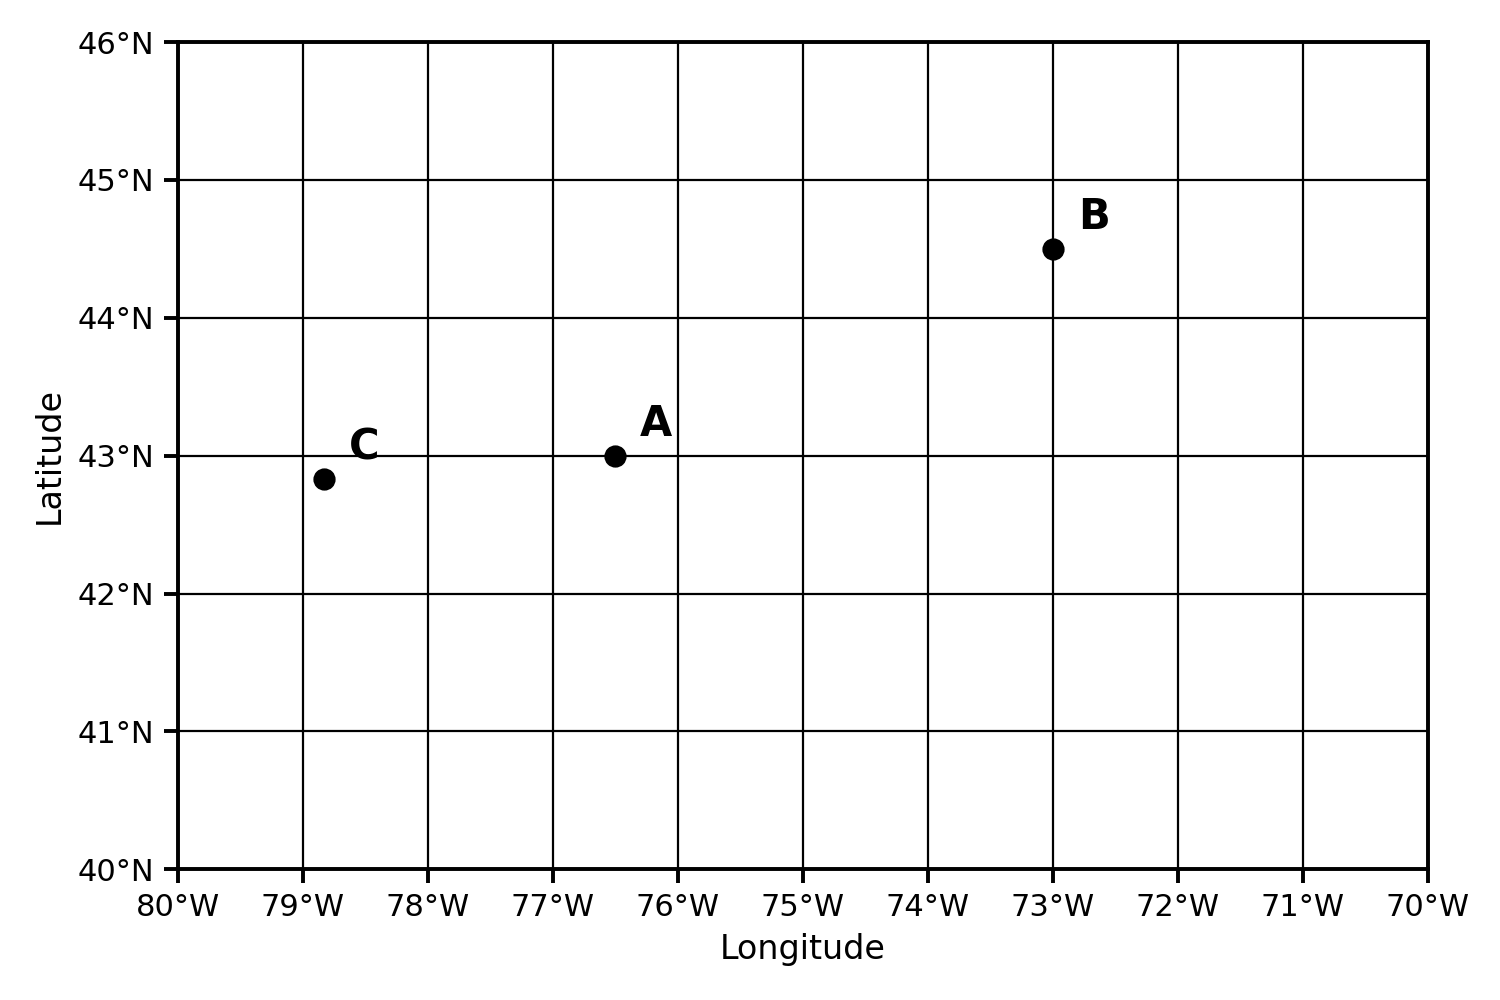
\includegraphics[width=0.78\linewidth]{grid-practice.png}
\end{center}

\vspace{-0.2\baselineskip}
\noindent\begin{tabular}{@{}p{0.5in}p{2.0in}p{2.0in}@{}}
 & \textbf{Latitude} & \textbf{Longitude} \\[2pt]
\textbf{A} & \midblank{43\dg00\mn\ N} & \midblank{76\dg30\mn\ W} \\[6pt]
\textbf{B} & \midblank{44\dg30\mn\ N} & \midblank{73\dg00\mn\ W} \\[6pt]
\textbf{C} & \midblank{42\dg50\mn\ N} & \midblank{78\dg50\mn\ W} \\
\end{tabular}

% ================================================================
\sectiontitle{5. Latitude and Polaris}

\noindent\begin{minipage}[t]{0.50\linewidth}
\vspace{0pt}
Polaris --- the \textbf{North Star} --- sits almost directly above Earth's
\blank{axis of rotation}.

\vspace{0.4\baselineskip}
Because of that, the \textbf{altitude} of Polaris (its angle above the horizon)
is equal to the observer's \blank{latitude}.

\vspace{0.4\baselineskip}
Polaris can only be seen from the \blank{Northern} Hemisphere.
\end{minipage}%
\hfill
\begin{minipage}[t]{0.47\linewidth}
\vspace{0pt}
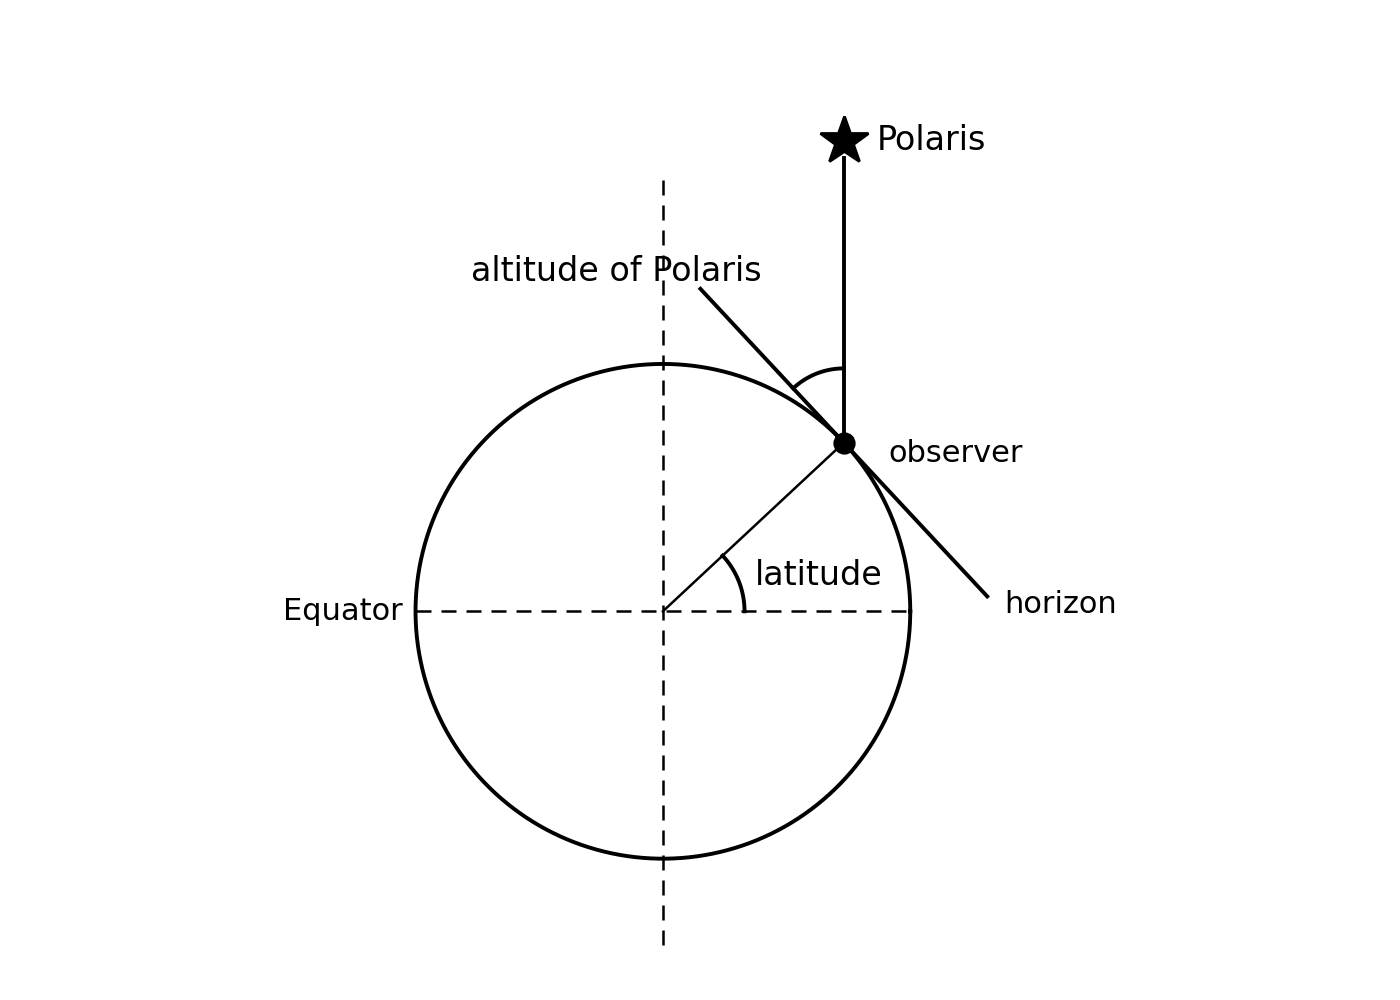
\includegraphics[width=\linewidth]{polaris-latitude.png}
\end{minipage}

\vspace{0.4\baselineskip}
\noindent\textbf{Check the extremes.} Fill in the altitude of Polaris at each location.

\vspace{0.2\baselineskip}
\noindent\begin{tabular}{@{}p{2.3in}p{1.6in}p{2.2in}@{}}
\hline
\textbf{Where you are} & \textbf{Latitude} & \textbf{Altitude of Polaris} \\
\hline
North Pole & 90\dg\ N & \tblblank{90\dg, overhead} \\[4pt]
Albany, NY & 42\dg\ N & \tblblank{42\dg} \\[4pt]
Equator & 0\dg & \tblblank{0\dg, on horizon} \\[4pt]
Southern Hemisphere & --- & \tblblank{not visible} \\
\hline
\end{tabular}

\vspace{0.5\baselineskip}
\noindent\textbf{Moving around.} Circle or fill in what happens to the altitude of Polaris.

\begin{itemize}[nosep,leftmargin=1.6em,itemsep=4pt]
  \item Travel \textbf{north}: Polaris gets \midblank{higher} and latitude \midblank{increases}.
  \item Travel \textbf{south}: Polaris gets \midblank{lower} and latitude \midblank{decreases}.
  \item Travel \textbf{east or west}: Polaris \midblank{does not change} and latitude \midblank{stays the same}.
\end{itemize}

\begin{keyidea}
Moving 1\dg\ of latitude changes the altitude of Polaris by exactly 1\dg\ ---
about 111 km (69 miles) of travel on the ground.
\end{keyidea}

% ================================================================
\sectiontitle{6. Longitude and time zones}

Meridians are counted east and west of the prime meridian until they meet at
\shortblank{180}\dg, which is called the \blank{Int'l Date Line}.

\[ \frac{360\dg \text{ of rotation}}{24 \text{ hours}} = \shortblank{15}\dg \text{ per hour} \]

\begin{keyidea}
Time zones are \shortblank{15}\dg\ of longitude wide, and each one represents
\midblank{1 hour} of time.
\end{keyidea}

\vspace{0.3\baselineskip}
\noindent Earth rotates from west to east, so places to the \textbf{east} rotate into
sunlight first and their clocks are \shortblank{ahead}. Places to the \textbf{west}
have clocks that are \shortblank{behind}.

\vspace{0.4\baselineskip}
\noindent\textbf{Worked example.} Albany is 74\dg\ W. Denver is 105\dg\ W.
How many hours apart are their clocks, and which is earlier?

\vspace{0.2\baselineskip}
\[ 105\dg - 74\dg = \shortblank{31\dg} \qquad \frac{31\dg}{15\dg/\text{h}} \approx \midblank{2 hours} \]

\noindent Denver is \textit{west} of Albany, so Denver's clock is
\blank{2 hours behind}.

% ================================================================
\sectiontitle{7. Check for understanding}

\begin{questions}

\question[1] The angle from the horizon to Polaris is equal to the \rule{0.9in}{0.4pt}
of the observer.
\begin{choices}
  \CorrectChoice latitude
  \choice longitude
\end{choices}

\question[1] Meridians are 15\dg\ apart, so time zones are separated by
\begin{choices}
  \choice 4 hours
  \choice 24 hours
  \CorrectChoice 1 hour
\end{choices}

\question[1] A ship sails due east across the Atlantic Ocean. The altitude of
Polaris will
\begin{choices}
  \choice increase
  \choice decrease
  \CorrectChoice stay the same
\end{choices}

\question[1] How many minutes are in 1\dg\ of latitude?
\begin{choices}
  \choice 10
  \CorrectChoice 60
  \choice 100
\end{choices}

\end{questions}

% ================================================================
\sectiontitle{Exit ticket}

\begin{questions}

\question[2] Using the \textit{Generalized Bedrock Geology of New York State} map in
your ESRT, give the latitude and longitude of Albany, NY to the nearest 10 minutes.

\begin{solutionorbox}[0.55in]
Approximately 42\dg40\mn\ N, 73\dg45\mn\ W.
\end{solutionorbox}

\question[2] An observer measures the altitude of Polaris as 30\dg. What is their
latitude, and which hemisphere are they in? Explain how you know the hemisphere.

\begin{solutionorbox}[0.85in]
They are at 30\dg\ N, in the Northern Hemisphere. Polaris cannot be seen at all
from the Southern Hemisphere, so any observer who can measure its altitude must be
north of the equator.
\end{solutionorbox}

\question[2] Explain in one sentence why time zones are 15\dg\ of longitude wide.

\begin{solutionorbox}[0.7in]
Earth rotates 360\dg\ in 24 hours, which works out to 15\dg\ per hour, so each
15\dg\ of longitude corresponds to one hour of time.
\end{solutionorbox}

\end{questions}

% ================================================================
\sectiontitle{Vocabulary}

\noindent\begin{tabular}{@{}p{1.5in}p{4.9in}@{}}
\textbf{Latitude} & angular distance north or south of the equator, 0\dg\ to 90\dg \\
\textbf{Longitude} & angular distance east or west of the prime meridian, 0\dg\ to 180\dg \\
\textbf{Equator} & the 0\dg\ line of latitude, halfway between the poles \\
\textbf{Prime meridian} & the 0\dg\ line of longitude, through Greenwich, England \\
\textbf{Parallel} & another name for a line of latitude \\
\textbf{Meridian} & another name for a line of longitude \\
\textbf{Altitude} & the angle of an object above the horizon \\
\textbf{Int'l Date Line} & the 180\dg\ meridian, where the calendar date changes \\
\end{tabular}

\end{document}
